\documentclass[main.tex]{subfiles}
\begin{document}

Since we will need to set arbitrary values for a lot of parameters, here are some values that will be useful.

\subsection*{k = 1}

We will very often need to use a distance parameter, for example a threshold to consider stations to be neighbors along a road. Thus it will be useful to know the distribution of the distances between 2 stations.
\begin{itemize}
    \item dist\_to\_k.min = 0
    \item dist\_to\_k.mean = 2 265
    \item dist\_to\_k.max = 17 087
\end{itemize}

\begin{figure}[H]
    \centering
    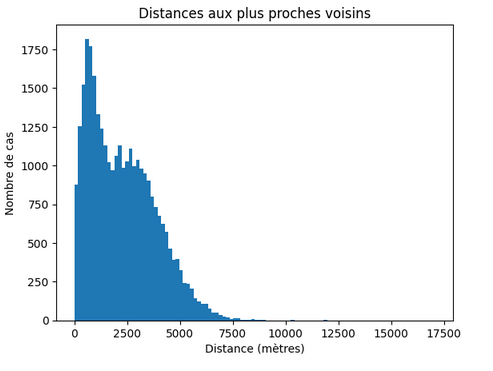
\includegraphics[width=0.5\textwidth]{Images/Didtrib_dist_1voisin.png}
    \caption{Distribution of the distance to the nearest neighbor}
\end{figure}

We will consider that the lowest values are probably in cities, and the highest (above 8000) are in the countryside, so the interval in which we will chose our parameters will be closer to [1000, 9000], depending of what we will need.

\subsection*{k = 15}

We will sometimes have to use KNN with higher values, and it will also be useful to know in these situations what values we can try arbitrarily for the distances. 
\begin{itemize}
    \item dist\_to\_k.min = 0
    \item dist\_to\_k.mean = 5 593
    \item dist\_to\_k.max = 32 891
\end{itemize}

\begin{figure}[H]
    \centering
    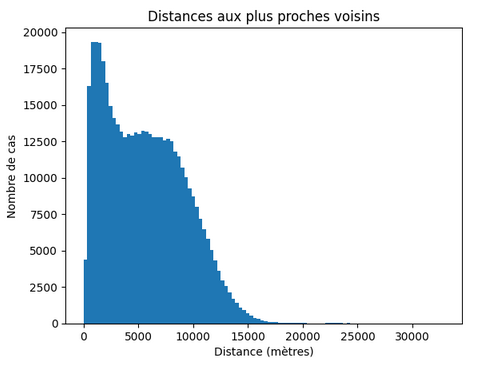
\includegraphics[width=0.5\textwidth]{Images/Didtrib_dist_15voisin.png}
    \caption{Distribution of the distance to the 15 nearest neighbors}
\end{figure}


\end{document}